% #############################################################################
% This is Chapter 1
% !TEX root = ../main.tex
% #############################################################################
% Change the Name of the Chapter i the following line
\fancychapter{Introduction}
\cleardoublepage
% The following line allows to ref this chapter
\label{chap:intro}
	
	The act of making things as perfect, functional, or effective as possible is a process known as optimization~\cite{MerriamWebster2017OptimizationDefinition}. Intuitively, through optimization one aims to improve a system's different quantitative measurable aspects. Although usually striving to fully optimize these systems, i.e., to obtain \textit{perfect} systems, in some cases, finding a better one or a near-optimal system suffices.
	
	Optimization has a paramount impact on decisions in the fields of economy, science, mechanics, engineering, among others. As a case in point, optimization yields a great potential to the architecture field, as it directly impacts the building industry: optimization enables the reduction of the economic and ecological footprint of the building sector through the finding of more efficient building variants, prior to their construction. 
	
	Modern architecture has grown to incorporate economic and environmental concerns into its building design practices by introducing standardized building regulations and energy certificates, among other limitations. These concerns led to new design approaches, like \ac{PBD} that seek for more efficient design solutions by considering the design's performance, possibly measured by using computational tools~\cite{Oxman2006PBD}.
	
	One example of the \ac{PBD} approach is the City Hall in London, shown in \Cref{fig:cityhalllondon}. The building was designed to achieve optimum energy performance by minimizing the surface area exposed to direct sunlight, thus originating its spherical-like form. The application of energy-saving techniques, such as leaning the building outwards so that the floorplates provide shading to the floors below, the use of groundwater from the water table to supply the building's cooling system, and the use of photovoltaic panels on the top of the building to maximize direct sunlight, enabled the reduction of the energy consumed by the building to be 75\% lower than the energy consumed by typical air-conditioned office buildings.
	
	\begin{figure}[htbp]
		\centering
		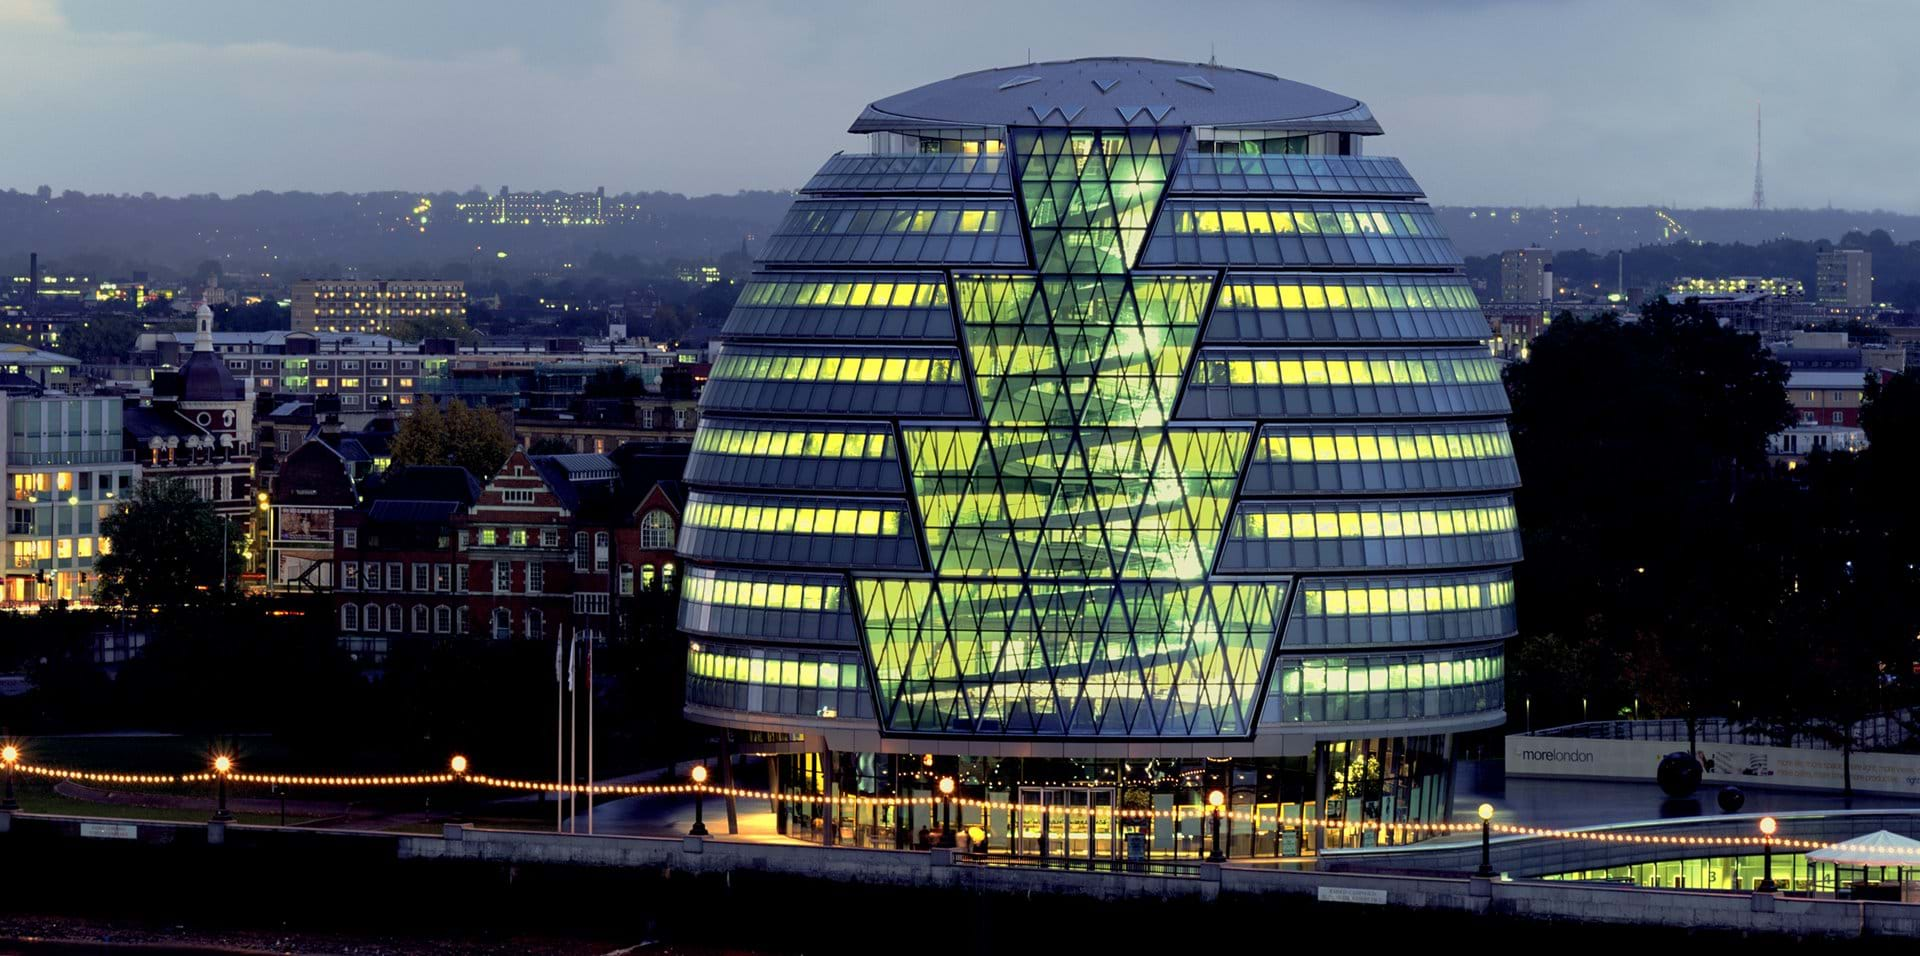
\includegraphics[width=0.70\textwidth]{./Images/Introduction/cityhalllondon.jpg}
		\caption{City Hall in London, designed by Foster and Partners}
		\label{fig:cityhalllondon}
	\end{figure}

	Notwithstanding the benefits attained with \ac{PBD}, to achieve the most performant designs regarding a certain aspect (e.g., lighting, thermal, structural, cost), these approaches evaluate multiple design variants. While a single evaluation may take up to several seconds, minutes, hours, or even days to complete, the time complexity becomes particularly problematic in building design, due to the existence of multiple conflicting aspects, e.g., maximum lighting and thermal comfort, and minimum energy consumption. In addition to the high time complexity associated with \ac{PBD} approaches, these also involve several manual decisions by architects and engineers.
		
	Given the importance of \ac{PBD} to the world's sustainability and economy, this dissertation  attempts to automate the \ac{PBD} process and, thus, enhance the architectural practice. To this end, we propose to study optimization algorithms especially targeted to solve problems involving expensive evaluation functions and to develop an automatic framework that supports their application within the architectural practice to create optimized designs. To better understand which algorithms to use and how to tackle \ac{PBD}'s time limitations, we must take its design process into consideration, namely, that it includes two main stages: the design and the analysis. While in the former, the architect creates a parametric design for which the parameters' values can be changed in order to obtain different design variants, in the latter, the architect evaluates a design's performance possibly by using analysis tools. This dissertation addresses the building performance optimization problem by repeatedly generating and evaluating different design variants, seeking for more efficient designs.
	
	The following sections of this chapter describe the evolution of the optimization practice in architecture, evidencing the limitations of different design processes and the foundations for the creation of an automatic optimization framework for architecture. Finally, we end by highlighting the dissertation's research goals and its structure.

%% #############################################################################
\section{From Design to Optimized Design}
	
	In architecture, optimization has been gaining relevance for the past few years, especially due to the impact of building construction and maintenance in the world's economy and environment~\cite{Attia2013, Shi2016}. For this reason, designers are now shifting from a purely aesthetically-based to \ac{PBD}, where buildings are optimized to achieve the best possible values regarding different characteristics of their design, such as thermal comfort, energy consumption, lighting comfort, structural behavior, cost, among others.

	This has only been possible due to the technological improvements in the architectural practice over the last few decades. The adoption of computer science techniques was responsible for the dissemination of digital modelling tools, which allowed for a more accurate and efficient design of highly complex buildings. These tools enabled the shift from traditional paper-based approaches to more computerized ones, such as \ac{CAD} and \ac{BIM} approaches, where changes to designs are facilitated, not requiring architects to manually erase and redraw parts of the original design~\cite{Ferreira2015GD}.~\Cref{fig:traditionaldesign} illustrates a general view of such computational design process, as well as an example of a 3D modeling tool. The architect interacts directly with the modeling tools to incrementally develop his design ideas.
	
\begin{figure*}[htbp]
\centering
\subfigure[]{%
\label{fig:traditionaldesign-a}%

\includegraphics[width=0.38\textwidth]{./Images/Introduction/TraditionalArchitecturalDesign.png}}%
\hfill
\subfigure[]{%
\label{fig:traditionaldesign-b}%
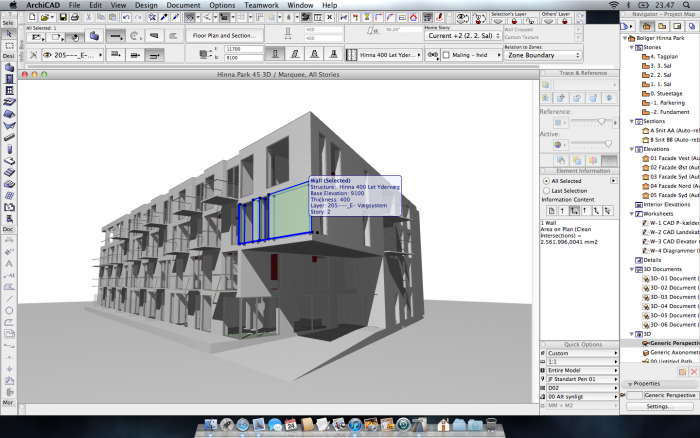
\includegraphics[width=0.48\textwidth]{./Images/Introduction/Example3DModellingTool_1.png}}%

\caption[General views of Traditional Design Approaches]{(a) Simplification of a computational design workflow (b) An example of a building design in a 3D modeling tool. Image retrieved from~\cite{3DMODELTOOL}}
\label{fig:traditionaldesign}
\end{figure*}

Shortly after, the development of computer-based simulation tools enabled designers to simulate the behavior of their designs regarding specific criteria, i.e., to get a measurement of its performance~\cite{Malkawi2005}. Through this process, known as \ac{BPS}, designers can easily validate whether their design's performance satisfies the efficiency requirements and, ultimately, optimize the design by iteratively generating multiple variations of it, assessing their performance, and selecting the better ones. Albeit still being very primitive, architects now have the elementary mechanisms required for optimizing their building's designs, which spurs a new \ac{PBD} approach.

% #############################################################################
\subsection{Building Performance Optimization}

	\ac{BPO}, a simulation-based optimization approach, treats the results produced by the simulation tool as the functions to optimize. Although invariably suffering from some degree of imprecision and inaccuracy, using these simulations made it possible to estimate the performance of complex designs. Particularly, these estimates are beneficial in designs for which analytical solutions are often very difficult or even impossible to derive~\cite{Kolda2003}. In these cases, the objective function, i.e., the function to optimize, is derived from the simulations' results. The domain of these functions corresponds to the range of acceptable designs,  which is specified by the architect.

	A known drawback of simulation-based approaches is the time required to achieve reasonable results for complex systems~\cite{Law1991} which is associated with different aspects of the problem, namely: (1) its \textbf{domain} which, depending on the nature of the problem, might use different methodologies to produce the corresponding estimates (e.g., thermal \textit{versus} structural); (2) its \textbf{intrinsic structure} that, depending on the attributes and relations of the system, might lead either to simpler or to more complicated computations (e.g., skyscraper \textit{versus} a small house); and (3) its \textbf{analytical model}, i.e., a model containing the essential properties of the system we are trying to simulate and that will be used as input to the simulation tool. Generally, the domain and structure do not change for the same problem, however there are numerous ways to produce multiple analytical models. Depending on the level of detail of the analytical model (e.g., using a single plane \textit{versus} a mesh to represent non-planar surfaces), both the computational time and results of the simulation might change. 

	In architecture, the generation of analytical models is a time-consuming and complex task. On the one hand, it is often necessary to generate multiple models of the same design because of the different simulation tools' specificities, i.e., each simulation tool requires its own specialized model of the same design. On the other hand, simulation tools often yield time-consuming processes, where a single simulation can take up to seconds, minutes, hours, days, or even weeks to complete. 
	
	In addition to the simulations' specificity and complexity, architectural designs are inherently complex, thus leading to less predictable objective functions for which mathematical forms are difficult to formulate~\cite{Machairas2014}. For this reason, information about the derivatives of such functions cannot be extracted and methods depending on function derivatives cannot be used to address architectural optimization problems. Particularly, classical gradient-based optimization methods cannot be used because they exploit the functions' derivatives. Instead, other methods that do not rely on the existence of an explicit mathematical form should be used, i.e., methods that treat the optimization functions as black-boxes, relying uniquely on the outputs of numerical simulations.
	
% Motivation for other design alternatives
	Finally, a \ac{BPO} methodology requires the evaluation of different design variations, which implies spending a large amount of time with the manual application of changes to the design. Despite the flexibility provided by \ac{CAD} and \ac{BIM} tools, architects often face difficulties when modeling complex geometry. As a result, the whole optimization process becomes unviable.
	
% #############################################################################
\subsection{Algorithmic Design}

% Introduction to AD, way of overcoming limitations of manual approaches
	A design approach capable of creating forms through algorithms is crucial for overcoming the aforementioned limitations. An example of such an approach is \ac{AD}~\cite{Branco2017AD} and \Cref{fig:algorithmicdesign} illustrates a simplified scheme of its application in the architectural design workflow. In this approach, the architect develops an algorithmic description of the intended design, that, when executed, generates the corresponding 3D model in an architectural modeling tool such as a \ac{CAD} or \ac{BIM} tool. Algorithmic approaches are inherently parametric, enabling the generation of different variations of the same design by simply modifying the parameters' values~\cite{Leitao2014GD}. 
	
\begin{figure}[htbp]
\centering

\includegraphics[width=0.70\textwidth]{./Images/Introduction/AlgorithmicArchitecturalDesign.png}
\caption[General view of the Algorithmic Design Approach]{Algorithmic Design workflow}
\label{fig:algorithmicdesign}
\end{figure}
	
	As an example, consider the algorithmic design of the Astana's National Library by Bjarke Ingels Group (BIG) architects illustrated in~\Cref{fig:astana-a}. Initially, the architect selects an \ac{AD} tool and, then, uses the available primitives to create a computational program enclosing the relationships between the different design elements, so that when a modification occurs in one element, that same modification is correctly propagated to the whole model. In the end, the architect creates a procedure responsible for creating the entire design, which in this case corresponds to the library's 3D model. Because the library's shape resembles a \textit{möbius} strip, its procedure is defined in terms of several parameters, amongst which the radius and the number of turns of the strip. Now, by invoking the procedure with different values for these parameters, the architect can easily generate different variations of the building. \Cref{fig:astana} illustrates the original design and two design variations, where the radius and number of turns parameters are increased, respectively. 
	
\begin{figure*}[htbp]
\centering
\subfigure[]{%
\label{fig:astana-a}%
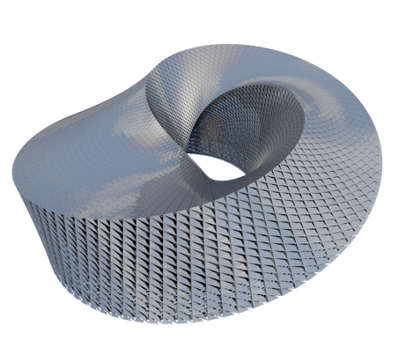
\includegraphics[width=0.32\textwidth]{./Images/Astana/Astana1.png}}%
\hfill
\subfigure[]{%
\label{fig:astana-b}%
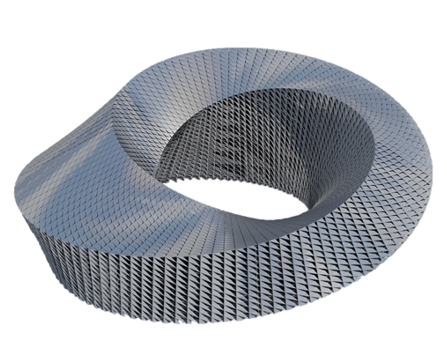
\includegraphics[width=0.33\textwidth]{./Images/Astana/Astana2.png}}%
\hfill
\subfigure[]{%
\label{fig:astana-c}%
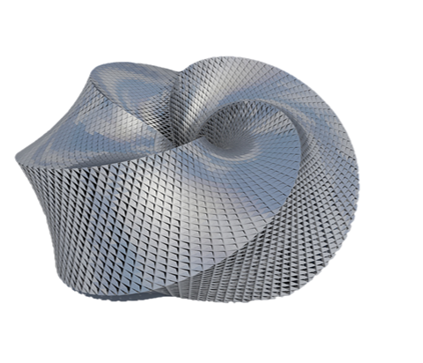
\includegraphics[width=0.33\textwidth]{./Images/Astana/Astana3.png}}%

\caption[Design variations of the Astana's National Library]{Design variations of the Astana National Library: (a) Original; (b) Larger diameter; (c) Two \textit{möbius} turns.}
\label{fig:astana}
\end{figure*}

% Advantages over Manual approaches & Disadvantages
Only recently has the algorithmic paradigm begun to settle in the architectural practice. The need for programming knowledge is often an obstacle to the adoption of these approaches, since it requires a large initial investment for architects to learn such techniques. Despite these investments, the benefits arising form the use of algorithmic design approaches surpass those of directly using \ac{CAD} or \ac{BIM} tools  to design complex buildings. Particularly, the initial investment is quickly recovered when the need for the incorporation of changes arises or when it becomes necessary to experiment different design variations~\cite{Leitao2014GD}. This is especially important when facing design processes that are characterized by constant changes to the project's constraints and requirements. In these scenarios, a manual-based approach requires constant manual changes to the model, thus incurring in a dreadful and tiresome process, whereas an algorithmic approach enables the effortlessly generation of a broader range of design solutions, as well as the easy modification of the models to comply with new requirements. As a result, using \ac{AD}, architects are able to explore larger regions of the design solution space, as well as innovative solutions that were not previously considered due to the time and effort required~\cite{Leitao2014GD}.

Another benefit of the \ac{AD} approach is the ease of maintenance of the models involved in building design. In fact, since \ac{AD} usually requires a single model of the design, the algorithmic model, it is easier to maintain in scenarios where changes are frequent. On the other hand, manual-based-approaches often involve the creation and maintenance of multiple models of the same design (e.g., analytical models, 3D models), which quickly becomes hard and tiresome.

% Conclusion
The emergence of \ac{AD} was crucial for the automation of optimization processes by enabling the automatic generation of multiple design solutions. However, the optimization of these designs requires the creation of the corresponding analytical models, which can be very dissimilar to the 3D models originally produced by the \ac{AD} tool. Therefore, to evaluate the \ac{AD} models produced by the \ac{AD} tool, the architect must manually generate the analytical model for each variation. Particularly, when dealing with complex buildings, this task requires a large amount of time and effort, which makes the optimization process almost impracticable.

% #############################################################################
\subsection{Algorithmic Analysis}

% Motivação p/ passar de AD p/ AA.
Faster and broader design space exploration prompted the creation of increasingly complex building designs, which became less predictable with respect to different aspects~\cite{Branco2017AD}, such as thermal, lighting, acoustics, among others. Moreover, the recent focus on efficient and sustainable buildings led to the demand for buildings that not only are well-designed, but also exhibit a good performance in those aspects.
	
% Motivar necessidade de ferramentas de tradução de modelos 
Nowadays, most of the available simulation-based analysis tools are single-domain, each one analyzing the parameters that are specific of the analysis domain~\cite{Malkawi2005}, i.e., while a lighting analysis tool measures daylight and glare coefficients, an energy simulation tool measures the coefficients related to thermal, energy consumption, ventilation, and air conditioning systems. Unfortunately, this often implies the production of different analytical models for the corresponding simulation tools. Moreover, the 3D models produced by the typically used modeling tools are generally dissimilar to the specialized models required by each analysis tool. To evaluate the design performance regarding different domains (e.g., lighting, energy, structural), several analytical models have to be produced either by hand or through translation processes that convert generic 3D models into specialized models required for analysis.

% Motivar processos automáticos para tradução 
Unfortunately, the process of producing analytical models is still limited: (1) hand-made analytical models require a considerable amount of time and effort to create; (2) the existing tools that attempt to convert a 3D model into its corresponding analytical model are frequently fragile and can cause errors or loss of information; (3) when using the analysis results to guide changes in the original design, such changes require additional time and effort to implement, as does redoing the analysis to confirm the improvements. For this reason performance analyses are typically postponed to later stages of the design process, only to verify the fulfillment of the performance requirements.

To overcome the limitations associated to the production of analytical models, one can exploit the idea of using \ac{AD} to automatically generate analytical models from the 3D model's algorithmic description. \ac{AA} is an extension of the \ac{AD} approach that, besides enabling the automatic generation of analytical models from a design's algorithmic description, also automates the setup of the analysis tool and the collection of its results~\cite{Aguiar2017}. Using this approach, the architect creates the \ac{AD} model reflecting his design's intents and then sets a few configuration parameters according to the analysis tool to be used. \Cref{fig:algorithmicanalysis} illustrates both the \ac{AD} and \ac{AA} design workflows, as well as examples of the Astana National Library models produced in each tool. Note that, even though there is only one algorithmic description of the design, it is capable of producing very different models for each given tool. As an example, consider the Astana National library's façade, which is composed of a truss structure holding the photostatic panels that cover the building. This façade is represented by a set of masses illustrating the geometry of the building in a typical 3D model, by a graph of truss bars, nodes, and edges when submitted to structural analysis, and by triangulated surfaces topped with sensor nodes, in the case of lighting analysis.

 % the produced models can be very different, e.g., while a truss is represented by a set of masses illustrating its bars and nodes in a typical 3D model, it is represented by a graph of nodes and edges when submitted to a structural analysis, and, by its surfaces, in the case of a lighting analysis.

\begin{figure}[htbp]
\centering
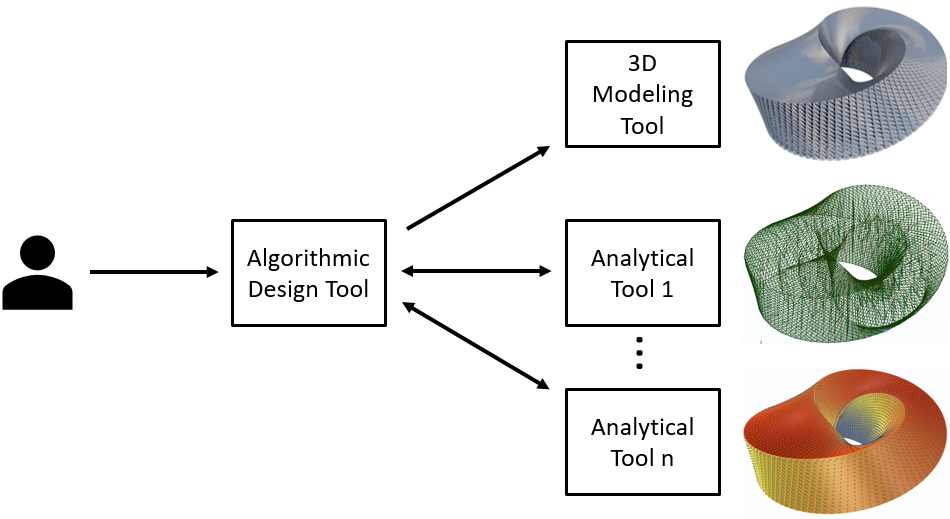
\includegraphics[width=1\textwidth]{./Images/Introduction/AlgorithmicDesignAndAnalysis_w_models2.png}
\caption[General view of the Algorithmic Design and Analysis approach]{\ac{AD} and \ac{AA} design workflow with examples of the Astana National Library design and analytical models: (top) 3D model; (center) structural analysis model (using Robot structural analysis tool); (bottom) pos-radiation analysis model (using Radiance analysis tool).}
\label{fig:algorithmicanalysis}
\end{figure}		
	
The \ac{AA} approach is able to enhance \ac{PBD} approaches, as it provides the means to effortlessly perform design analysis throughout the whole design process, instead of just at final stages. Depending on the performance requirements, architects might need to use different analysis tools: (1) for daylight analysis, Daysim and Radiance are very popular tools among the community, (2) for energy simulations, EnergyPlus, TRNSYS and DOE-2 are widely used~\cite{Nguyen2014}, (3) for structural analysis, Robot Structural analysis is a well-known reputed tool, and (4) for acoustic analysis, Olive Tree Lab and Pachyderm Acoustical Simulation are examples of good tools.%~\cite{Branco2017AD}. 

The \ac{AA} approach is also very important for the automation of optimization processes, as it abstracts the production of the analytical model, removing the need for direct human intervention, while reducing the occurrence of errors and information loss. Additionally, when combined with \ac{AD}, it provides the required mechanisms to quickly update a design, to generate the corresponding analytical model, to automatically evaluate the design in an analytical tool, and, finally, to collect the results and use them to guide the search for optimal solutions. 

Despite the possibility of automating optimization processes, in order to do so, every time  architects intend to improve a design, they must create a script including an optimization algorithm. As a result, architects are either forced to create their own algorithms or to use the ones existing in other dedicated optimization software, such as the MATLAB toolbox, GenOpt among others. On the one hand, creating their own algorithm requires programming skills that architects usually do not possess and, even if they succeed in its creation, due to the large amount of effort involved, they will often be tempted to adopt the same algorithm to optimize all their designs. While this is not always a disadvantage, it can have a drastic impact in the overall optimization time if, for example, architects systematically apply algorithms with bad performance. On the other hand, while being substantially better than the previous approach, the available optimization tools still lack post-processing and visualization features. In an attempt to fill these gaps and obtain interpretable results, architects often created ad-hoc scripts to integrate the optimization software with existing post-processing tools, like DView, Excel, gnuplot, which due to the tools' specificity, often represented an obstacle to the optimization process itself. Among other obstacles, the lack of programming knowledge, as well as the large amount of time and investement required to implement automated optimization processes are often the main setbacks to its application in the architectural design context~\cite{Attia2013}. 

Notwithstanding its obstacles, optimization prevailed and different approaches have spawned into the architectural practice. During this time, multiple surveys have identified the difficulties and the advantages of each approach, which enabled the development of optimization tools more targeted to architect's needs. In the following section, we briefly mention some of these approaches and we emphasize the key points of optimization processes in architecture.
	
% #############################################################################
\subsection{Architectural Optimization Workflow}
	
 More recently, the emergence of \ac{AD} approaches based on visual programming techniques, such as Grasshopper and Dynamo~\cite{GRASSHOPPER,DYNAMOBIM}, together with the growing consciousness of both the limitations and benefits of optimizating building designs, led to the development of ready-to-use optimization toolsets (e.g., Galapagos, Opossum). However, despite enabling the optimization of several designs, such parametric design tools are known to scale poorly with the complexity of the design~\cite{Heijden2015}, thus diminishing and restricting its optimization capabilities. 

On the other hand, \ac{AD} approaches, based on textual programming techniques, are known to scale well with design complexity. In addition to the scalability benefits, its growing popularity among building design practitioners~\cite{Kestelier2013}, its flexibility and capacity to automate optimization processes allow the development of more robust and complete optimization tools. To fully benefit from these properties, the architect must follow an optimization methodology based in \ac{AD}, where he first idealizes a design and, then creates the corresponding algorithmic program by defining the parameters that represent the degrees of freedom of the design\todo{Inserir aqui a falar de PBDG ? e a referenciar anexo}, i.e., the parameters that he is willing to manipulate. After the algorithmic definition of the model, the \ac{AD} tool generates either a 3D or an analytical model for visualization and performance analysis purposes, respectively. Optionally, the architect may decide to optimize his design according to some particular performance aspects (e.g., lighting, energy consumption, cost), potentially leading to the exploration of design solutions that were not previously considered. In that case, the optimization algorithm explores different design candidates, using the results produced by the simulation tools as the functions to optimize. The execution of the optimization algorithm then yields optimal (or near optimal) design solutions.

Considering the previous view of an algorithmic-based design workflow, we identify four key dimensions in an optimization process:

% ------- BEGIN \ --------
\begin{enumerate}
% ANALYTICAL MODELS
\item \textbf{Analytical models}: when the optimization algorithm specifies a candidate design, i.e., a concrete configuration for the parameters of the model, analytical models are automatically generated by the \ac{AD} tool and then used as input for the corresponding analysis tools. These models can be improved either through simplification of the analytical models or by enriching them with context information. The former enables the simplification of the analysis itself by providing an equivalent but simpler model to the tool, and potentially reducing the simulation time, whilst the latter enables the attainment of more detailed and realistic simulations, which is not always possible due to limitations in the \ac{AD} tool. 

% OPTIMIZATION ALGORITHM
\item \textbf{Optimization algorithms}: the algorithms used to explore the design space in the quest for optimal (or near optimal) solutions. These algorithms use the results obtained in the performance analysis of different design variations as the functions to optimize, i.e., objective functions. Generally, optimization algorithms use the inferred functions to guide the search for optimal solutions. The algorithm's time complexity typically depends on the number of times these funcitons are evaluated. In architectural design, these functions entail time-intensive simulations, thus instilling optimization processes that may take minutes, hours, days, or even weeks to complete.

% EXPLAINABILITY / INTELLIGIBILITY OF RESULTS
\item \textbf{Intelligibility of results}: the ability to interpret and understand the design optimization results is very important within the architectural community \cite{Shi2016,Cichocka2017SURVEY}. Having access to an explanation regarding the quality of a solution allows architects to make more informed design decisions. In this way, not only can the architect provide valuable arguments for its implementation, but he also can learn with the process, depending on the quality of the explanations, thus fostering more efficient and faster future designs. 

% INTERACTIVITY AND VISUALIZATION
\item \textbf{Interactivity and visualization}: interactive and visual aspects are highly important features in the context of optimization processes~\cite{Ashour2015CreativelyMOO}. On the one hand, an interactive optimization process enables the architect to use knowledge about the problem at hand, for instance, by adding or removing constraints or by exploring different, yet unexplored regions of the design space, hence potentially increasing the process' performance. On the other hand, optimization processes providing better visualizations and representations of their own evolution can present their users with better feedback about the course of the search. This feedback is important to the comparison of variable-objective correlations and the making of more informed design decisions about the optimization process itself, e.g., whether the evaluations made so far suffice or if the algorithm is converging to non-conventional designs that diverge from the original design intent.
\end{enumerate}


% #############################################################################
\section{Dissertation Goals}

This dissertation focus on optimization problems involving expensive evaluation functions, namely, in the context of building design. Despite the evident benefits of architectural design optimization, its application within the architectural community remains punctual. This might be explained due to the its considerable time complexity, since most design practices are time sensitive~\cite{Shi2016}. Time becomes an even greater impediment when it becomes necessary to evaluate multiple performance aspects, instead of a single aspect. Since building design often requires the evaluation of multiple aspects simultaneously, it is of paramount importance that the optimization algorithms used for optimizing designs are capable of efficiently handle problems involving costly evaluations. Unfortunately, this is not the case, as the algorithms provided by currently available architectural tools do not, in general, provide good algorithms for handling time-consuming problems.

This dissertation sets to address this problem, by studying and exploring different optimization algorithms capable of handling computationally complex problems more efficiently and how they can be applied to architectural design optimization problems. The goal is, then, to consider not only building design problems involving a single performance aspect, i.e., \ac{SOO} problems, but also to approach the recurrent practice of simultaneously evaluating multiple aspects, that is, the \ac{MOO} problems. Based on the idea that no algorithm that can consistently perform better than the others on all problems~\cite{Wolpert1997NFLT}, this dissertation explores this performance difference by studying algorithms with different properties and classifications. 

In this dissertation, we propose an optimization framework that allows the usage of different optimization algorithms to search for more efficient building designs regarding multiple performance aspects
\todo{Não gosto desta frase... não percebo o q significa em concreto...}. To evaluate the viability of the proposed framework in the architectural practice and to study the algorithms' behaviors, a prototype will be implemented and tested on several real \ac{BPO} problems. 

Finally, we draw some conclusions regarding the behavior and the suitability of the studied algorithms for handling time-consuming design problems, such as building design ones, and we compare the framework proposed in this dissertation with the currently existing ones. \todo{Melhorar *sigh*...}


% #############################################################################
\section{Document Structure}
The following chapters are organized as follows: \\ 
% \textbf{\Cref{chap:intro}} discusses optimization concepts and evidences its importance for different problems, ranging from simple day-to-day decisions to more complex engineering problems, such as components, circuits, and building designs. Particularly, this chapter stresses the relevance of optimization in the architectural context, providing a comprehensive overview of the existing practices and the difficulties underlying the adoption of optimization processes in architecture. \\
\textbf{\Cref{chap:back}} presents an overview of the current optimization practices in architecture and makes a balance of the benefits and drawbacks associated to each one.  \\
\textbf{\Cref{chap:architecture}} describes the architecture of the implemented framework and enumerates important design decisions that were made during its implementation. \\
\textbf{\Cref{chap:implement}} \todo{ADD one chapter about the implementation...} \\
\textbf{\Cref{chap:evaluation}} evaluates both quantitative and qualitative aspects of the proposed solution, evaluating its performance in the context of three real case studies. \\
\textbf{\Cref{chap:conclusion}} emphasizes the importance of optimization in architecture and draws some conclusions about this work and how it can effectively influence the architectural practice. Finally, we reflect on the future improvements for the proposed framework. \\
